%<*figPipeline>
\begin{figure*}
	\centering
	\scalebox{0.9}{
		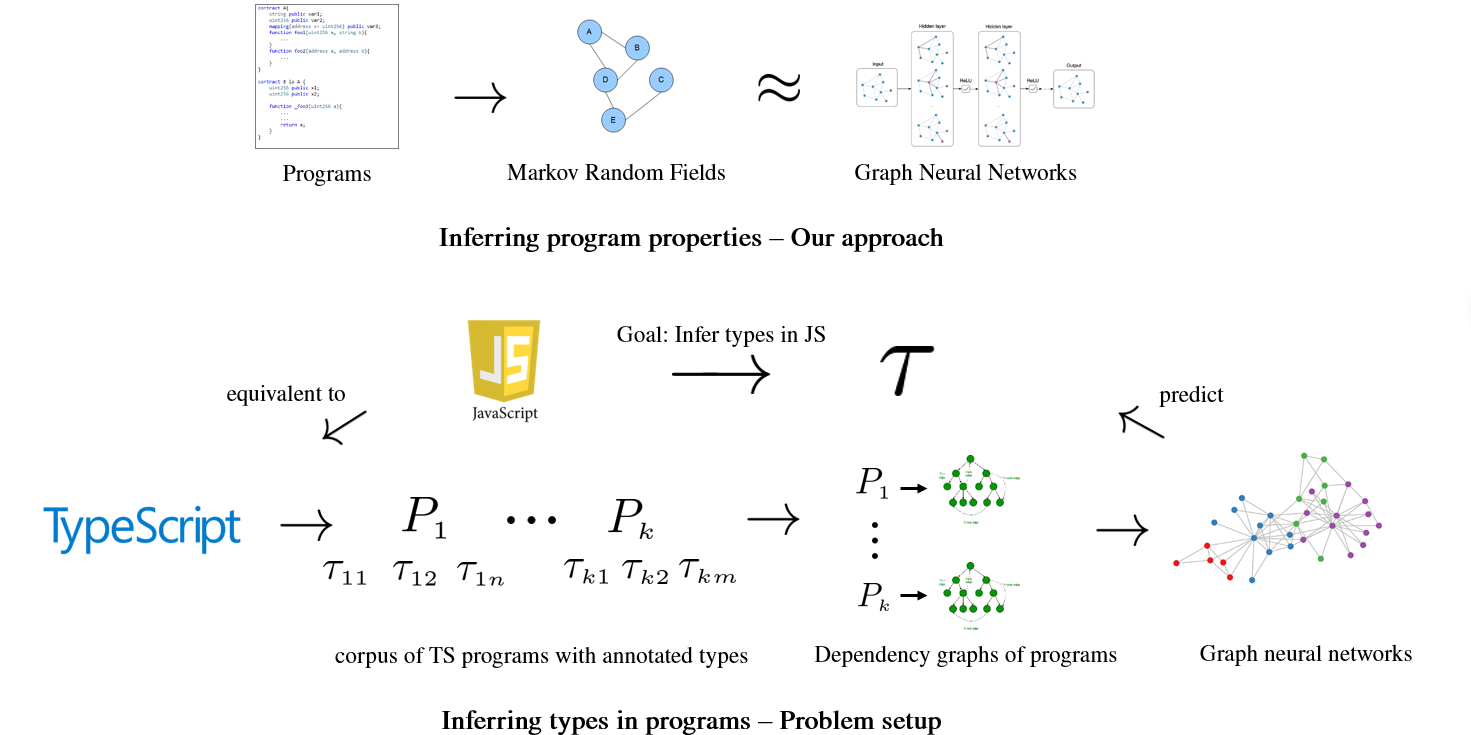
\includegraphics[width=\textwidth]{img/architecture.png}
	}
	\caption{\textbf{Summary of our work.} We motivate the problem of modeling programs as Markov Random Fields. We argue that a Graph neural network approximates inference tasks over an MRF. Specifically, we investigate the problem of inferring types in Javascript programs.}
	\label{fig:pipeline}
\end{figure*}
%</figPipeline>

%<*figSetup>
\begin{figure}
	\centering
	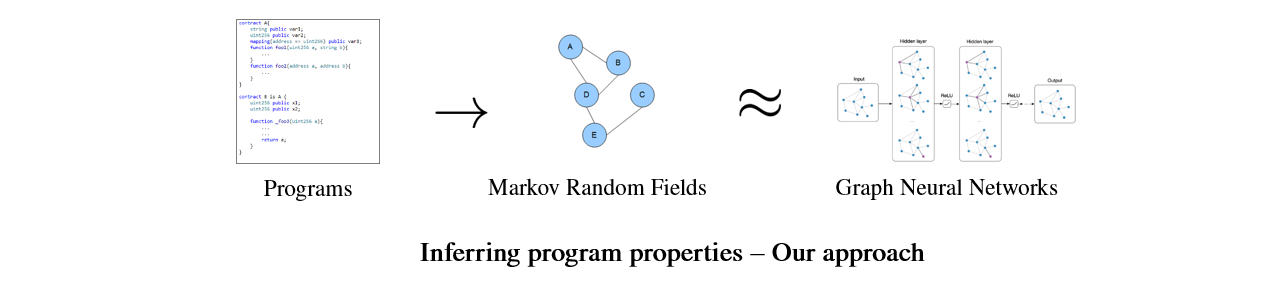
\includegraphics[width=\linewidth]{img/approach.png}
	\caption{Problem setup}
	\label{fig:setup}
\end{figure}
%</figSetup>

%<*gnn>
\begin{figure}
	\centering
	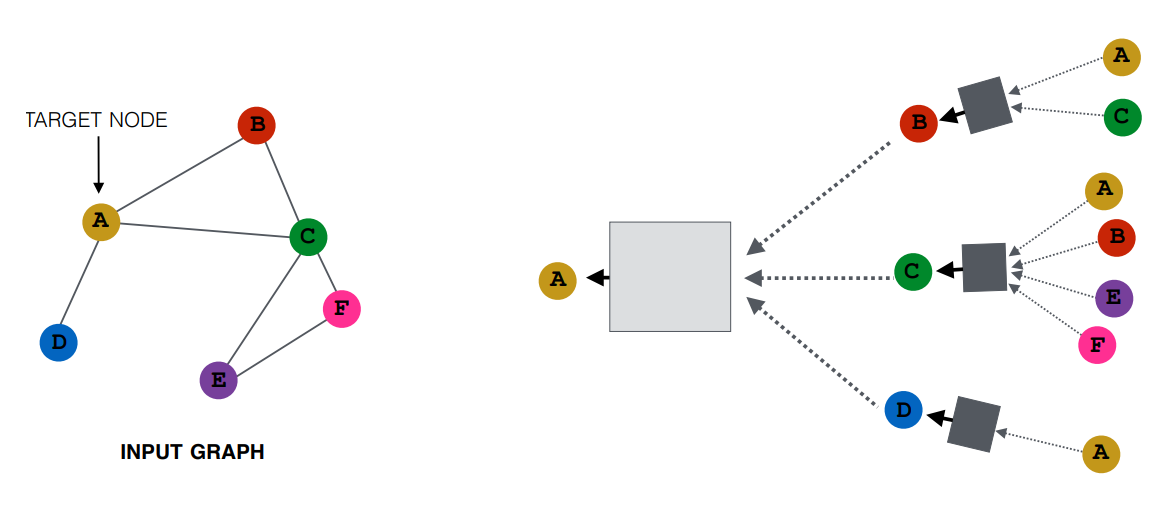
\includegraphics[width=\linewidth]{img/gnn.png}
	\caption{A typical graph neural network architecture. The key idea is to generate node embeddings based on neighborhood information. Image credit: Tutorial slides from \textit{Representation Learning on Networks}, held at WWW 2018.}
	\label{fig:gnn}
\end{figure}
%</gnn>



%<*figUseDefCombined>
\begin{figure}[!t]
	\centering
	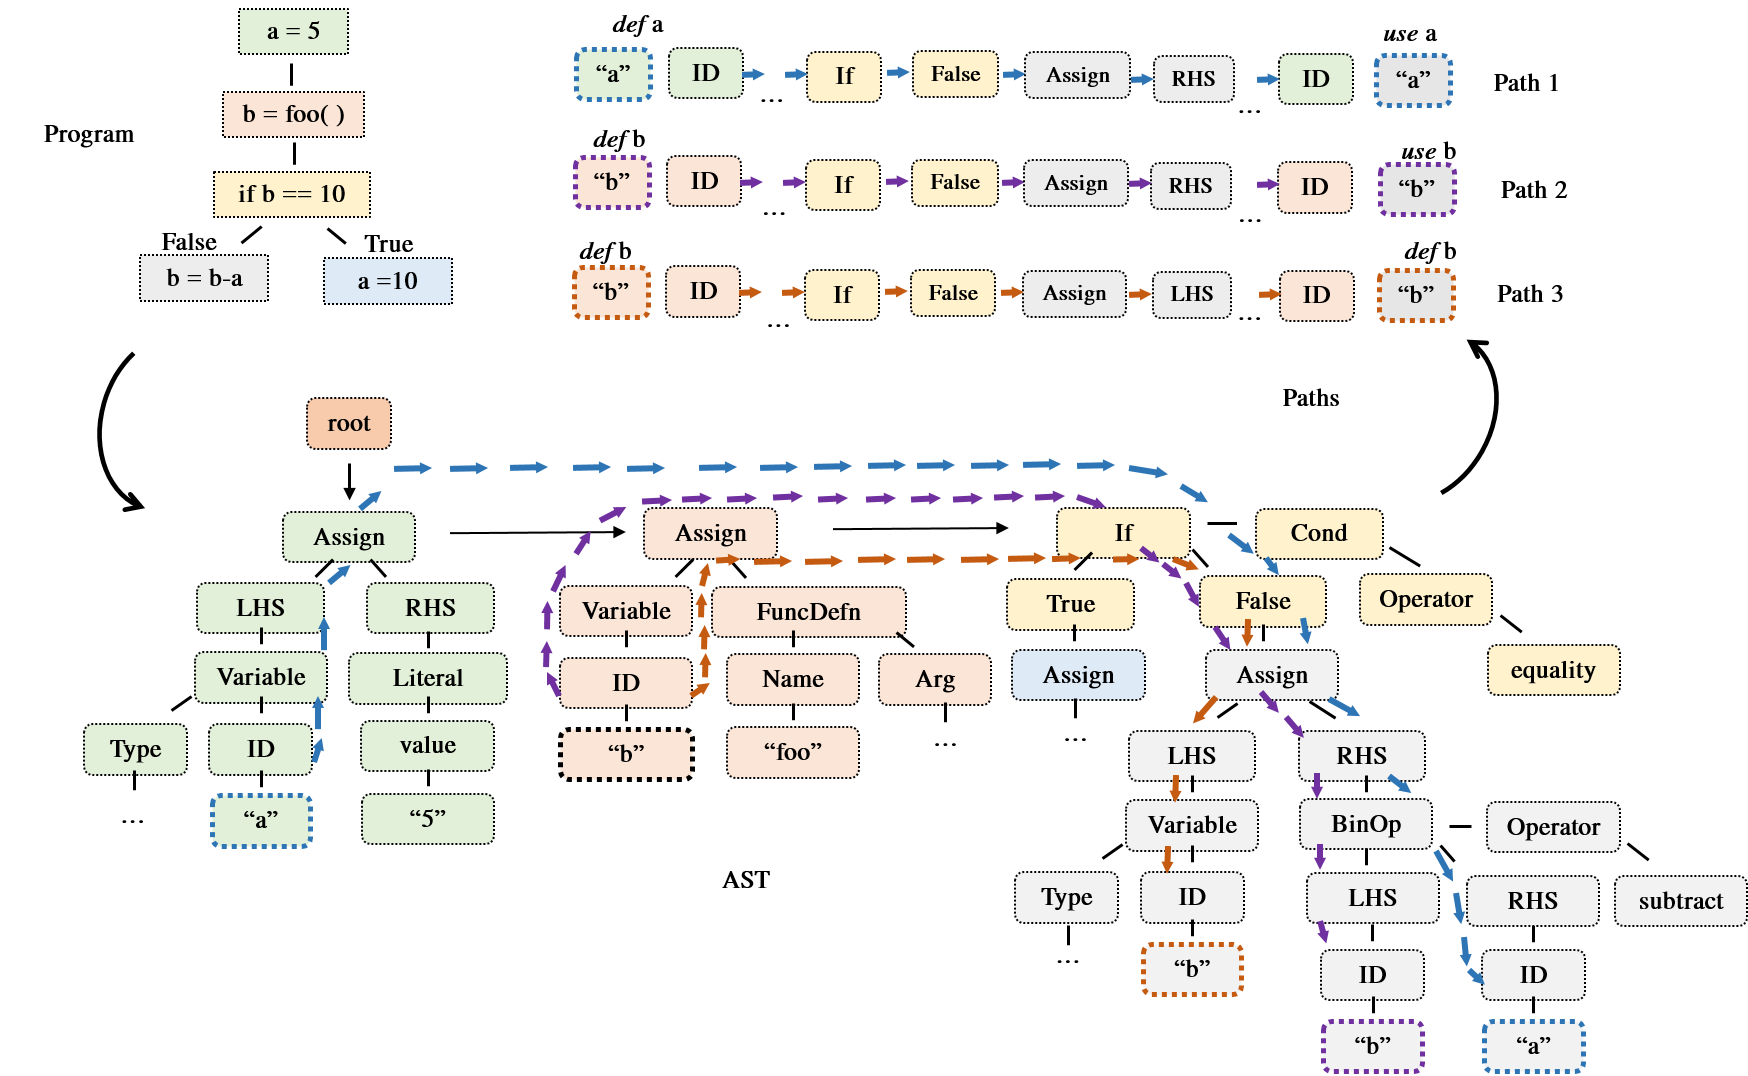
\includegraphics[scale=0.3]{img/ast.png}
	\caption{\usedef Paths - An example. Paths to the expression
		$\;b=b-a$ are shown. Statements and their corresponding sub-trees have been shaded in the same color.}
	\label{fig:use_def_combined}
\end{figure}
%</figUseDefCombined>


%%% Local Variables:
%%% TeX-master: "main"
%%% End: